\chapter{\textsf{ETVA}}
\section{Descrição}
A Eurotux Virtual Appliance é uma ferramenta de gestão centralizada de recursos disponíveis numa rede. Consiste numa distribuição linux pré-instalada e configurada que permite fazer a gestão via rede de servidores e seus recursos.


A ETVA encontra-se dividida principalmente em dois blocos funcionais:

\begin{itemize}
	\item \emph{Central Management} (CM)
        \item \emph{Virtualization Agent} (VA)
\end{itemize}

\begin{figure}[H]
	\begin{center}
	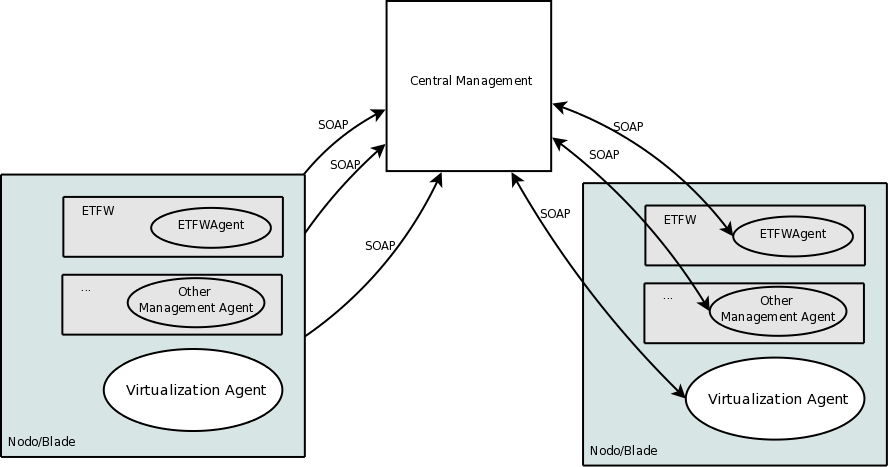
\includegraphics[scale=0.35]{screenshots/etva_blocos.png}
	\caption{Esquema geral do ETVA}
	\label{fig:etva_blocos}
	\end{center}
\end{figure}

O \textsf{CM} é o bloco responsável por gerir toda a infra-estrutura.
Os \emph{Virtualization Agents} são responsáveis pelo processamento dos pedidos entre os servidores de virtualização (\emph{Nodes}) e o CM.

Dentro de um servidor de virtualização(\emph{Node}) poderão existir máquinas virtuais com \emph{Management Agents}. Estes agentes, permitem a gestão ao nível dos serviços/aplicações instalados numa máquina virtual (ver Figura \ref{fig:etva_blocos} ).

\section{Versões}

Actualmente o ETVA encontra-se disponível em duas versões:
\begin{description}
	\item[Standard -] Nesta versão o modelo do ETVA consiste num único servidor de virtualização onde se encontram instalados o CM e o VA. A configuração de rede neste modelo consistem em quatro redes: Internet, LAN, DZM e Management.
		\begin{figure}[H]
			\begin{center}
			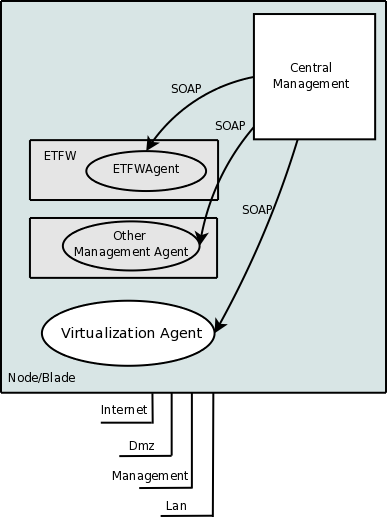
\includegraphics[scale=0.4]{screenshots/etva_standard.png}
			\caption{Modelo ETVA Standard}
			\label{fig:etva_standard}
			\end{center}
		\end{figure}
	\item[Enterprise -] Nesta versão existem vários servidores de virtualização a comunicar com o CM. A configuração da rede inicial, é efectuada, com recurso a VLANs, através do Assistente de configuração inicial conforme indica a Figura \ref{fig:first_time_wizard}.
		\begin{figure}[H]
			\begin{center}
			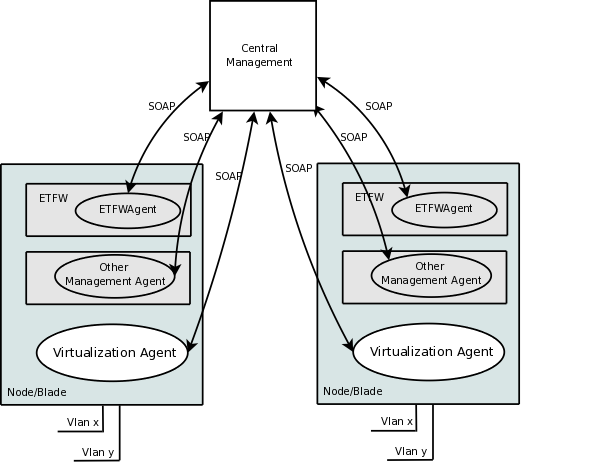
\includegraphics[scale=0.6]{screenshots/etva_enterprise.png}
			\caption{Modelo ETVA Enterprise}
			\label{fig:etva_enterprise}
			\end{center}
		\end{figure}
\end{description}
 
Este manual de utilização/configuração descreve a ferramenta de gestão do ETVA, o \textsf{CM}.

\pagebreak

\chapter{\textsf{ETVA Central Management}}

\section{Estrutura da interface principal}
O layout principal é constituido por quatro áreas:

\begin{description}
	\item[Painel topo -] Contem menus de acesso a acções do sistema, tais como a administração de utilizadores, gestão de ISOs e visualização das mensagens do sistema.
	\item[Painel esquerdo (\emph{Nodes}) -] Lista as máquinas reais/servidores de virtualização - {\bf\emph{nodes}} e as máquinas virtuais associadas a cada \emph{node} - {\bf\emph{servers}}. No nível imediatamente abaixo de \emph{Main} encontram-se os vários servidores de virtualização registados no CM. As funcionalidades permitidas num servidor de virtualização estão descritas na secção \ref{sec:node}. No nível abaixo de um \emph{node} encontram-se as máquinas virtuais do respectivo \emph{node}. As funcionalidades de uma máquina virtual encontram-se descritas na secção \ref{sec:server}. Ao clicar em cada item é carregada a informação correspondente no painel principal.
	\item[Painel principal -] Área onde é visualizada o conteúdo pretendido, consoante o contexto (item a visualizar).
	\item[Painel de informação (\emph{Info Panel}) -] Área de breve notificação acerca dos eventos despoletados pelo utilizador. Mensagens de erro e sucesso são aqui visualizadas.
\end{description}

\begin{figure}[H]
	\begin{center}
	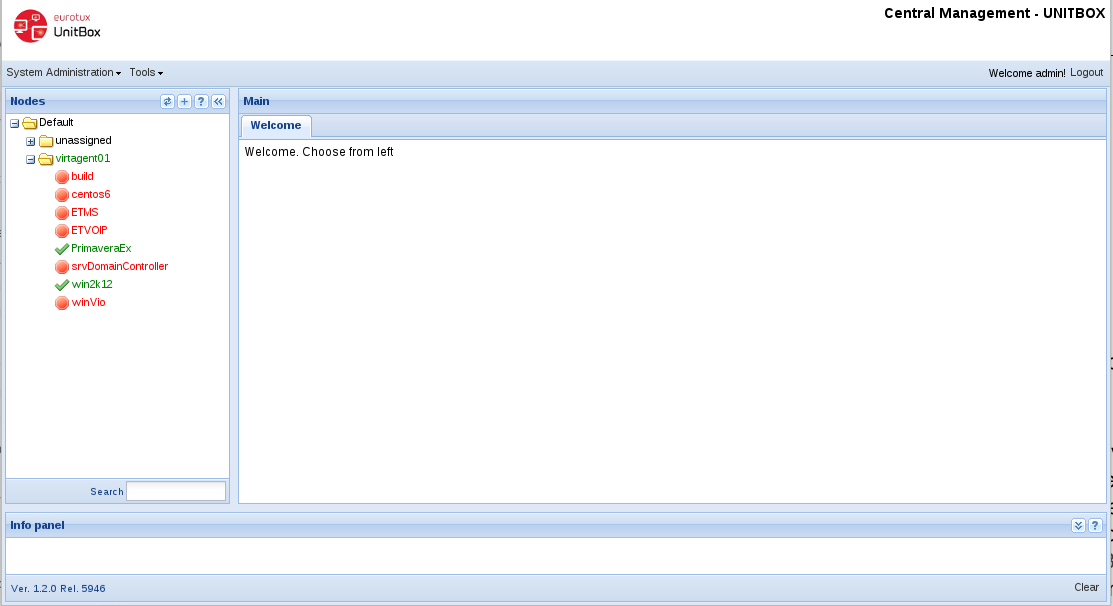
\includegraphics[scale=0.5]{screenshots/principal.png}
	\caption{Layout principal}
	\label{fig:principal}
	\end{center}
\end{figure}

\pagebreak


\section{Primeiro acesso}

Após a instalação do CM pela primeira vez acede-se ao url do sistema disponível no endereço http://<IP>/\footnote{Endereço da máquina onde se encontra instalado o CM.}

\begin{figure}[H]
	\begin{center}
	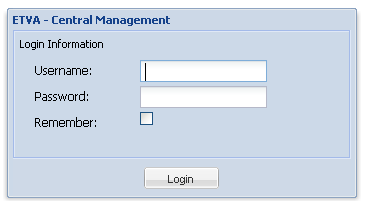
\includegraphics[scale=0.7]{screenshots/login.png}
	\caption{Página de autenticação}
	\label{fig:login}
	\end{center}
\end{figure}

Após a abertura da página \emph{Web} deverá ser introduzido o \emph{Username} e a respectiva \emph{Password}.

\begin{quote}
	{\large \bf Nota} \\*[-.8pc]
	\underline{\hspace{6in}} \\
	Ao instalar o CM pela primeira vez as credenciais de acesso são:
	\begin{description}
        	\item[Username:] admin
	        \item[Password:] admin
	\end{description}
	Por questões de segurança recomenda-se a alteração da password do sistema no primeiro acesso.

\begin{figure}[H]
        \begin{center}
        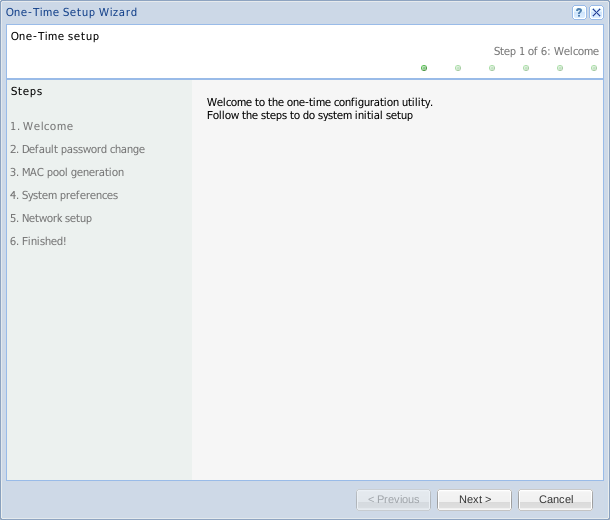
\includegraphics[scale=0.7]{screenshots/first_time_wizard.png}
        \caption{Assistente de configuração inicial ({\bf ETVA Enterprise})}
        \label{fig:first_time_wizard}
        \end{center}
\end{figure}

\end{quote}

No primeiro acesso ao Central Management deverá surgir o Assistente de configuração inicial.

A configuração inicial consiste nos seguintes passos:
\begin{itemize}
	\item Alteração da password inicial
	\item Geração da MAC pool	
	\item Configuração das Redes
\end{itemize}

Caso se trate de um {\bf ETVA Standard} é omitida a configuração das redes.

De seguida, e após a instalação e configuração de um agente virtualização num \emph{node}, este regista-se automáticamente no CM, passando o CM a dispor de mais funcionalidades.
No painel esquerdo, \emph{Nodes} (ver figura \ref{fig:principal}), surgirá o servidor de virtualização registado no CM e poderá então passar-se a efectuar a gestão desse \emph{node} conforme as opções descritas na secção \ref{sec:node}.

\pagebreak

\section{Main}

Neste painel é apresentada a vista geral do CM.
Podemos visualizar os servidores de virtualização e a informação da rede do CM (ver figura \ref{fig:main_nodes}).

\subsection{Nodes}

Em \emph{Nodes} é disponibilizada alguma informação acerca dos vários servidores de virtualização. Podemos ver o \emph{hypervisor} suportado pelas máquinas reais e, entre outras informações, o estado do agente de virtualização.
\begin{figure}[H]
	\begin{center}
	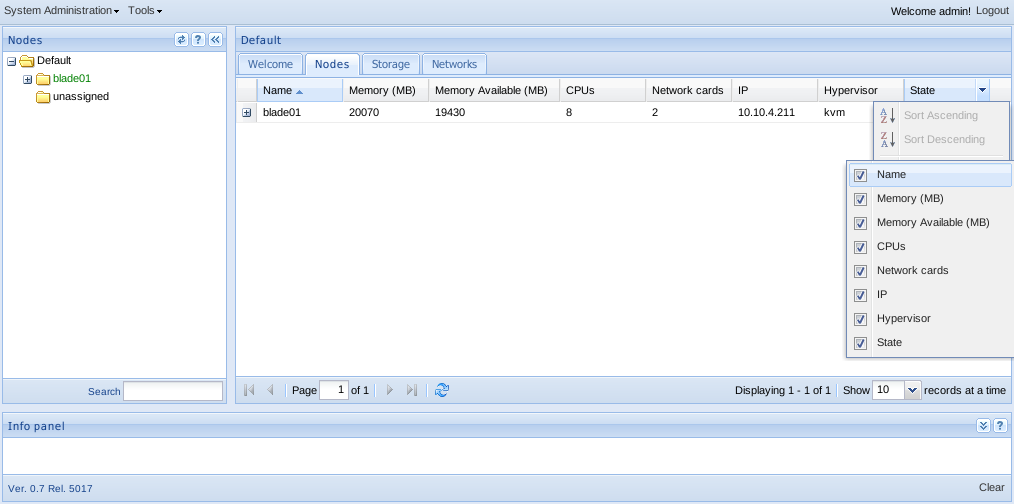
\includegraphics[scale=0.5]{screenshots/main_nodes.png}
	\caption{Vista dos nodes do Central Management}
	\label{fig:main_nodes}
	\end{center}
\end{figure}

\subsection{Networks}

Este painel permite efectuar as seguintes operações sobre o CM:

\begin{itemize}
	\item Administração das Redes do sistema
	\item Gestão da pool de MAC Addresses
	\item Gestão das interfaces de rede das máquinas virtuais 
\end{itemize}

\begin{figure}[H]
	\begin{center}
	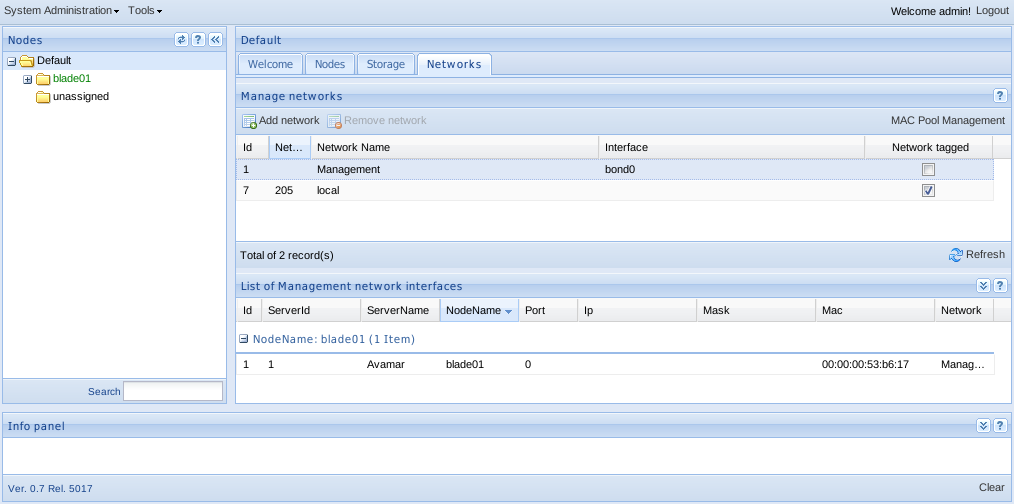
\includegraphics[scale=0.5]{screenshots/main_networks.png}
	\caption{Vista das redes do sistema  e das interfaces de rede}
	\label{fig:main_networks}
	\end{center}
\end{figure}

É possível também filtrar as interface de rede numa determinada rede clicando sobre a rede pretendida conforme a figura \ref{fig:main_networks}.
Na figura \ref{fig:main_networks} as interfaces de rede listadas são as que estão associadas à rede \emph{Internet}

\subsubsection{Adicionar Rede}
\label{sec:network_create}

\begin{quote}
	{\large \bf Nota} \\*[-.8pc]
	\underline{\hspace{6in}} \\
	Esta opção só está disponivel na versão ETVA Enterprise.
\end{quote}

Para criar uma rede clica-se em \emph{Add Network}.
A informação da Rede consiste no seu nome e ID\footnote{Caso a rede/vlan seja \emph{tagged} o campo \emph{ID} refere-se à {VLAN ID}}.

\begin{figure}[H]
	\begin{center}
	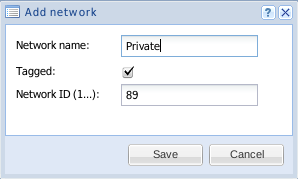
\includegraphics[scale=0.5]{screenshots/network_create.png}
	\caption{Janela de criação de uma Rede}
	\label{fig:network_create}
	\end{center}
\end{figure}
A Rede adicionada é propagada a todos os \emph{nodes} do CM.

\subsubsection{Gestão da pools de MAC Addresses}
\label{sec:mac_pool}

Em \emph{MAC Pool Management} (ver figura \ref{fig:main_networks}), é possivel criar a pool de MAC Addresses.
Para além de adicionar MACs à pool, pode-se visualizar as redes associadas e os MACs ainda disponíveis da pool.

\begin{figure}[H]
	\begin{center}
	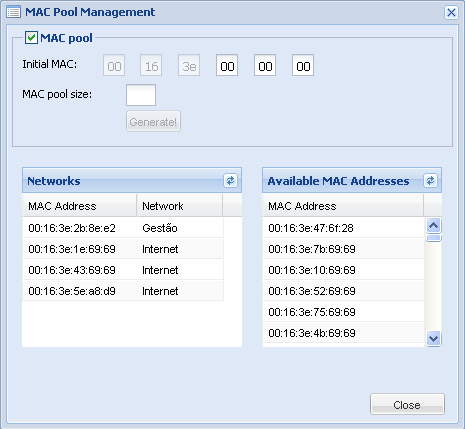
\includegraphics[scale=0.5]{screenshots/networks_macpool.png}
	\caption{Janela de criação da pool de MAC's}
	\label{fig:networks_macpool}
	\end{center}
\end{figure}


\subsubsection{Gestão das interfaces de rede das máquinas virtuais}
Seleccionando um registo da tabela de Interfaces e acedendo ao sub-menu de contexto, é possível remover a interface de rede associada a esse registo - \emph{Remove interface}, ou alterar as placas de rede associadas à máquina virtual associada ao registo seleccionado - \emph{Manage Interfaces}.

\begin{figure}[H]
	\begin{center}
	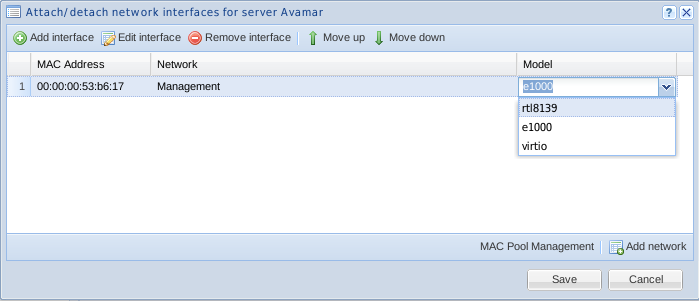
\includegraphics[scale=0.5]{screenshots/nics.png}
	\caption{Adicionar/Remover NIC's de uma máquina virtual}
	\label{fig:nics}
	\end{center}
\end{figure}

% PAINEL NODE

\section{Servidor de virtualização}
\label{sec:node}

No painel \emph{Nodes} é possivel seleccionar um \emph{node}(servidor de virtualização) e efectuar operações sobre ele como:
\begin{itemize}
    \item Visualizar informação do \emph{node} (ver secção \ref{sec:nodeinfo})
    \item Gestão de máquinas virtuais (ver secção \ref{sec:servers})
    \item Gestão da storage do node (ver secção \ref{sec:storage})
\end{itemize}

\subsection{Node info}
\label{sec:nodeinfo}
Em \emph{Node Info} é disponibilizada a informação acerca do servidor de virtualização. Podemos ver o \emph{hypervisor} suportado pela máquina real e, entre outras informações, o estado do agente de virtualização.

\begin{figure}[H]
	\begin{center}
	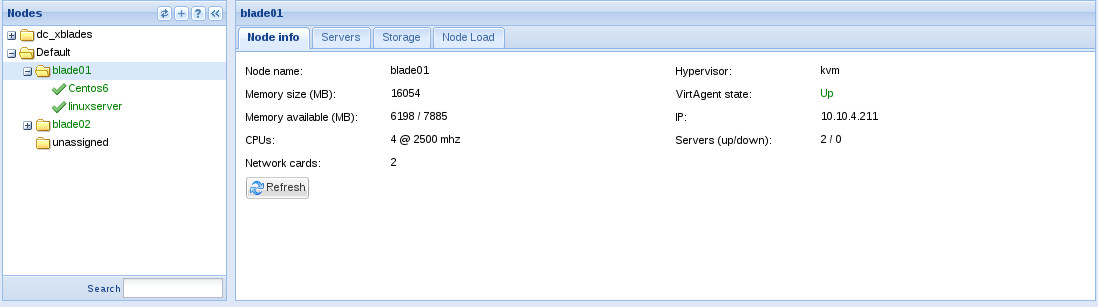
\includegraphics[scale=0.5]{screenshots/node_info.png}
	\caption{Informação do node \emph{VirtAgent01}}
	\label{fig:node_info}
	\end{center}
\end{figure}

\subsection{Servers}
\label{sec:servers}
Em \emph{Servers} é disponibilizada a informação ácerca das máquinas virtuais existente no servidor de virtualização. Para além de visualizar informação, este painel permite efectuar as seguintes operações:
\begin{itemize}
	\item Adicionar máquina virtual
	\item Remover maquina virtual
	\item Abrir máquina virtual numa consola VNC
	\item Iniciar/parar máquina virtual
    \item Migrar máquina virtual
\end{itemize}
\begin{figure}[H]
	\begin{center}
	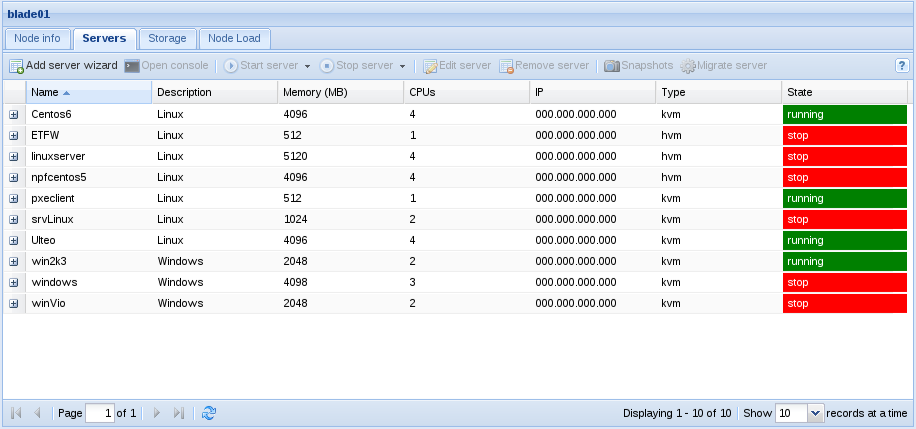
\includegraphics[scale=0.5]{screenshots/node_servers.png}
	\caption{Lista das máquinas virtuais de um node}
	\label{fig:node_servers}
	\end{center}
\end{figure}

\subsubsection{Adicionar máquina virtual (server)}
\label{sec:add_server}

Para adicionar uma nova máquina virtual utiliza-se o botão \emph{Add Server Wizard}.
\begin{quote}
	{\large \bf Nota} \\*[-.8pc]
	\underline{\hspace{6in}} \\
	Esta opção só se encontra activa se o agente de virtualização estiver a correr no \emph{node} (máquina real) e este conseguir estabelecer comunicação com o CM.
\end{quote}
 

\begin{figure}[H]
	\begin{center}
	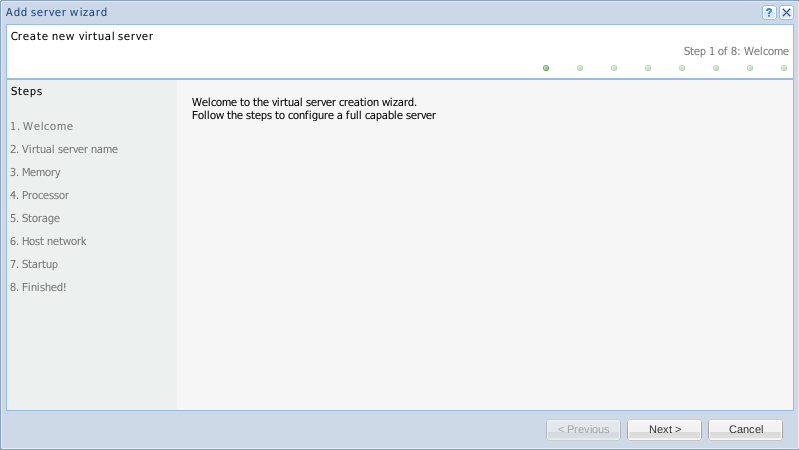
\includegraphics[scale=0.5]{screenshots/server_createwiz.png}
	\caption{Server Wizard - Welcome}
	\label{fig:server_createwiz}
	\end{center}
\end{figure}
O wizard é constituido pelas seguintes etapas:
\begin{description}
	\item[Virtual server name:] Nesta etapa define-se o nome da máquina virtual e o tipo de sistema operativo. As opções do sistema operativo variam consoante a especificação do node:
		\begin{itemize}
			\item com XEN e suporte a virtualização por hardware:
			\begin{itemize}
				\item Linux PV
				\item Linux HVM
				\item Windows
			\end{itemize}
 			\item com XEN sem suporte de virtualização por hardware:
			\begin{itemize}
				\item Linux PV
			\end{itemize}
 			\item com KVM
			\begin{itemize}
				\item Linux
				\item Windows
			\end{itemize}
		\end{itemize}
	
		\begin{figure}[H]
        		\begin{center}
		        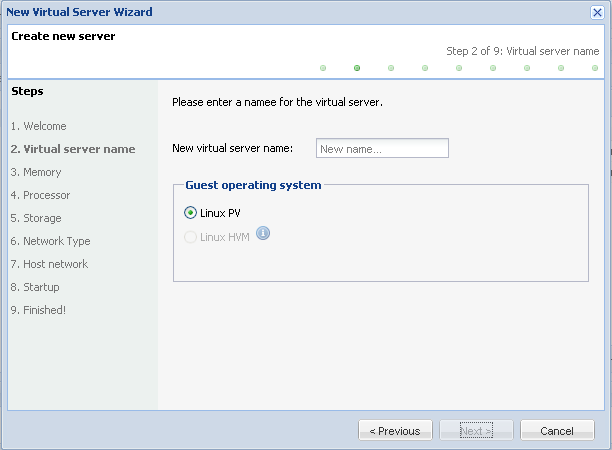
\includegraphics[scale=0.5]{screenshots/server_createwiz_name.png}
        		\caption{Server Wizard - Virtual Server name}
	        	\label{fig:server_createwiz_name}
	        	\end{center}
		\end{figure}
 
	\item[Memory:] Especificação da memória a ser usada pela máquina.
		\begin{figure}[H]
        		\begin{center}
		        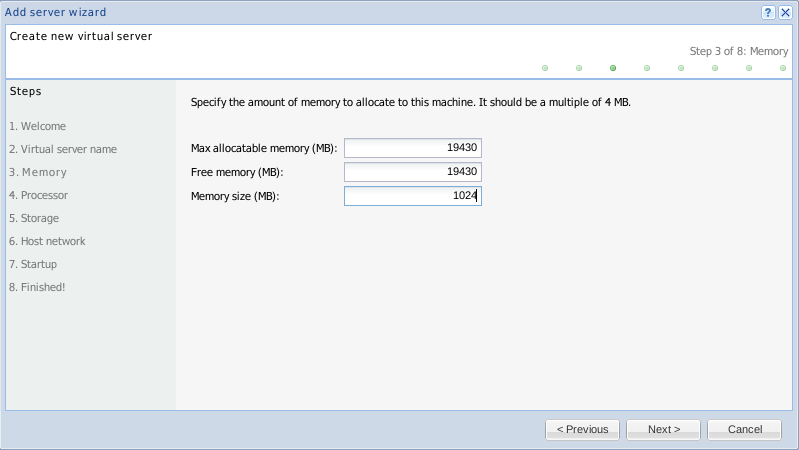
\includegraphics[scale=0.5]{screenshots/server_createwiz_memory.png}
        		\caption{Server Wizard - Memory}
	        	\label{fig:server_createwiz_memory}
	        	\end{center}
		\end{figure}

	\item[Processor:] Nesta etapa define-se o número de processadores a usar.
		\begin{figure}[H]
        		\begin{center}
		        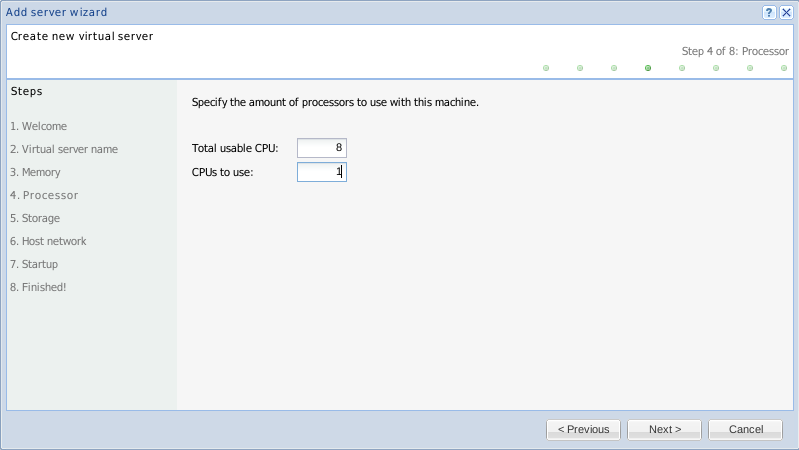
\includegraphics[scale=0.5]{screenshots/server_createwiz_processor.png}
        		\caption{Server Wizard - Processor}
		        \label{fig:server_createwiz_processor}
	        	\end{center}
		\end{figure}

	\item[Storage:] Define o disco de arranque da máquina virtual. Pode ser uma das três opções:
\begin{itemize}
	\item usar um logical volume/ficheiro já existente - \emph{Existing logical volume}
	\item criar um novo logical volume/ficheiro (para criar um ficheiro através desta opção tem que se seleccionar o volume group \emph{\_\_DISK\_\_}\footnote{Ver secção \ref{sec:storage}}) - \emph{New logical volume}
	\item  ou caso pretenda criar um ficheiro usar a opção \emph{New disk file} que para tal necessita apenas do nome e tamanho.
\end{itemize}

		\begin{quote}
			{\large \bf Nota} \\*[-.8pc]
			\underline{\hspace{6in}} \\
			Se o node não suportar physical volumes a opção \emph{Existing logical volume} será desabilitada, uma vez que não é possivel criar logical volumes, mas sim apenas ficheiros (disk file).
		\end{quote}
	
		\begin{figure}[H]
        		\begin{center}
	        	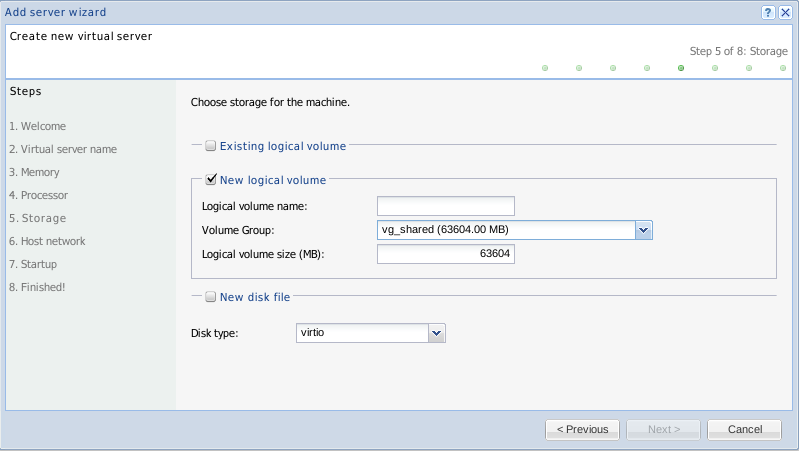
\includegraphics[scale=0.5]{screenshots/server_createwiz_storage.png}
	        	\caption{Server Wizard - Storage}
		        \label{fig:server_createwiz_storage}
        		\end{center}
		\end{figure}

        \item[Network Type:] Especificação da ligação da máquina virtual à rede.
		\begin{itemize}
			\item Use bridged networking\\
			Modo usado por omissão. A máquina virtual fica visível em toda a rede, e pode ser vista por outras máquinas na rede.
			\item Use network address\\
			Network Address Translation - NAT
			\item Use host-only\\
			Usado para criar uma rede privada com várias máquinas virtuais sem ser necessário o uso de interfaces de rede físicas. Cria interfaces de rede virtuais permitindo ter conectividade entre as  máquinas virtuais e o node.
		\end{itemize}
		
		\begin{figure}[H]
        		\begin{center}
	        	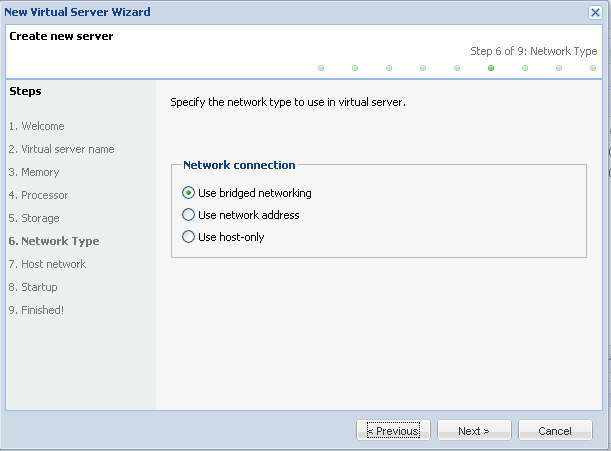
\includegraphics[scale=0.5]{screenshots/server_createwiz_nettype.png}
	        	\caption{Server Wizard - Network Type}
		        \label{fig:server_createwiz_nettype}
        		\end{center}
		\end{figure}
        
	\item[Host network:] Especificação das interfaces de rede existentes no \emph{server}. Caso não existam endereços MAC disponíveis é possível criar através de \emph{Add MAC Pool}. Igualmente para as redes é possível criar nesta etapa através de \emph{Add Network}.
		\begin{figure}[H]
        		\begin{center}
	        	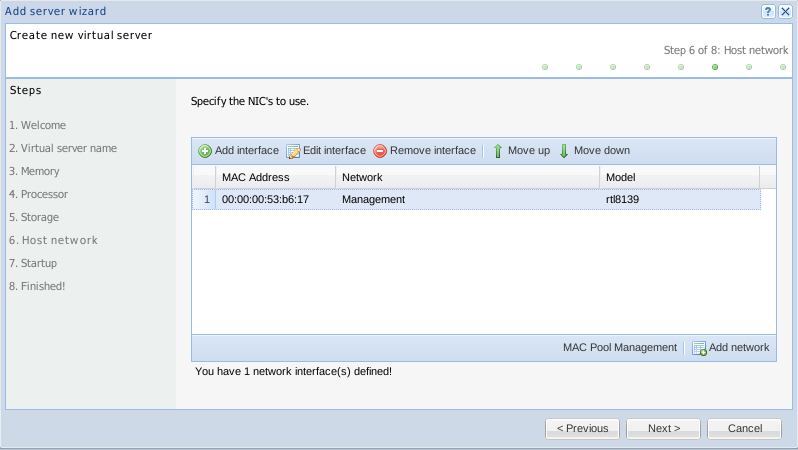
\includegraphics[scale=0.5]{screenshots/server_createwiz_hostnet.png}
	        	\caption{Server Wizard - Host network}
		        \label{fig:server_createwiz_hostnet}
        		\end{center}
		\end{figure}

        \item[Startup:] Especificação de parâmetros de arranque da máquina virtual. As opções nesta etapa variam consoante o tipo de sistema definido na etapa \emph{Virtual server name}:
		\begin{itemize}
			\item \emph{Linux PV}
				\begin{itemize}
					\item Network install location. Url do kernel a carregar.
				\end{itemize}
			\item Outros
				\begin{itemize}
					\item Network boot (PXE)
					\item CD-ROM (ISO)
				\end{itemize}
		\end{itemize}
A figura \ref{fig:server_createwiz_startup} refere-se às opções de uma máquina virtual em \emph{Linux PV}.

		\begin{figure}[H]
			\begin{center}
			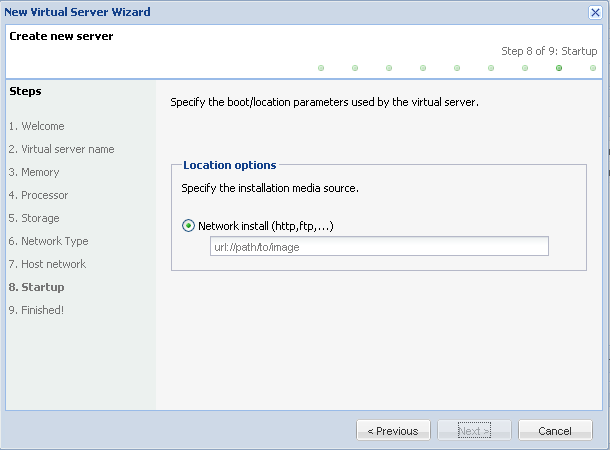
\includegraphics[scale=0.5]{screenshots/server_createwiz_startup.png}
			\caption{Server Wizard - Startup}
			\label{fig:server_createwiz_startup}
			\end{center}
		\end{figure}

	\item[Finished!] Etapa final do \emph{wizard}. Após confirmação da criação do server, a máquina é criada no node. Posteriormente no painel \emph{Servers} poderá ser arrancada a máquina através da opção \emph{Start Server}.
		\begin{figure}[H]
			\begin{center}
			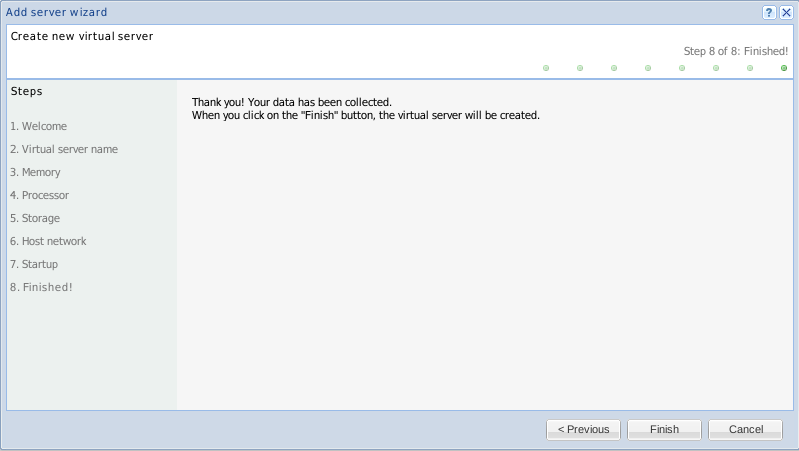
\includegraphics[scale=0.5]{screenshots/server_createwiz_finish.png}
			\caption{Server Wizard - Finished!}
			\label{fig:server_createwiz_finish}
			\end{center}
		\end{figure}

\end{description}

\subsubsection{Remover máquina virtual}
\label{sec:remove_server}
Para remover um \emph{server}, selecciona-se a máquina a remover e clica-se em \emph{Remove Server}.

A opção \emph{Keep disk file} permite manter o disco associado à máquina aquando da sua criação, caso contrário será também removido.
		
\begin{figure}[H]
	\begin{center}
	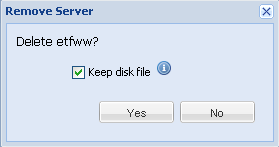
\includegraphics[scale=0.5]{screenshots/server_remove.png}
	\caption{Janela de remoção de um server}
	\label{fig:server_remove}
	\end{center}
\end{figure}

\subsubsection{Abrir máquina virtual numa consola VNC}
\label{sec:open_vnc}

Seleccionando um \emph{server} e de seguida clicando em \emph{Open Console} é possível estabelecer uma ligação VNC com a máquina, desde que esta esteja a correr.

\begin{quote}
	{\large \bf Nota} \\*[-.8pc]
	\underline{\hspace{6in}} \\
	Caso o input do teclado esteja desconfigurado é possível alterar o \emph{keymap} do VNC através da opção \emph{Set keymap} no sub-menu de contexto do painel \emph{Nodes}.
\end{quote}

\subsubsection{Iniciar/parar máquina virtual}
\label{sec:start_server}

No arranque da máquina virtual é possível escolher um dos seguintes parâmetro de boot:
\begin{description}
	\item[VM Filesystem:] Arranque pelo disco associado ao \emph{server}.
    	\item[Location URL:] Arranque pelo url definido em Location\footnote{Só disponível caso o tipo da máquina virtual seja \emph{Linux PV}}.
	\item[CD-ROM:] Arranque pela ISO montada no CD-ROM\footnote{Só disponível caso o tipo da máquina virtual não seja \emph{Linux PV}}.
    	 
\end{description}

\begin{figure}[H]
	\begin{center}
	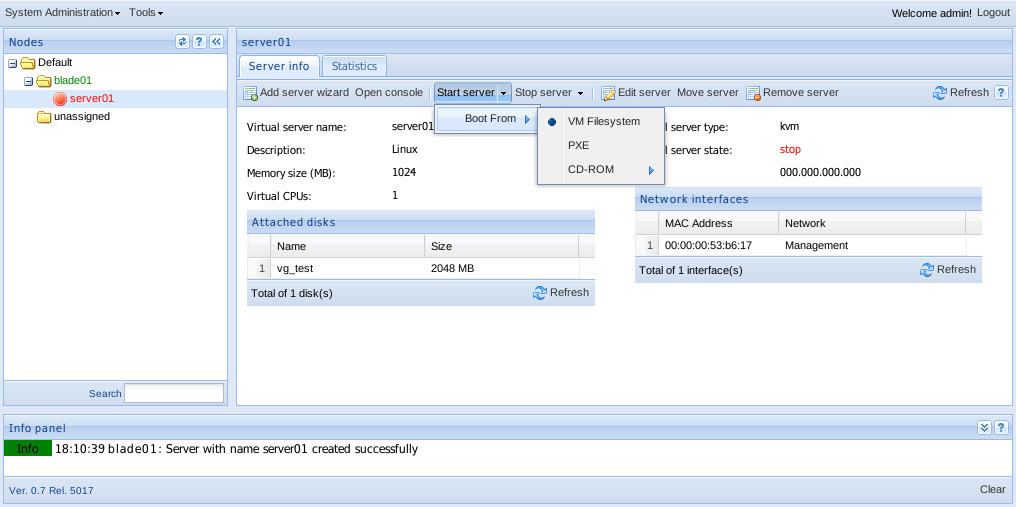
\includegraphics[scale=0.5]{screenshots/server_start.png}
	\caption{Parâmetros de arranque de uma máquina virtual}
	\label{fig:server_start}
	\end{center}
\end{figure}


\subsubsection{Migrar máquina virtual}
\label{sec:migrate_server}

Seleccionando um \emph{server} e de seguida clicando em \emph{Migrate server} é possível migrar uma máquina de um \emph{node} para outro desde que partilhem a mesma \emph{storage}.
A migração de uma máquina virtual é efectuada no modo \emph{offline}.

\begin{figure}[H]
	\begin{center}
	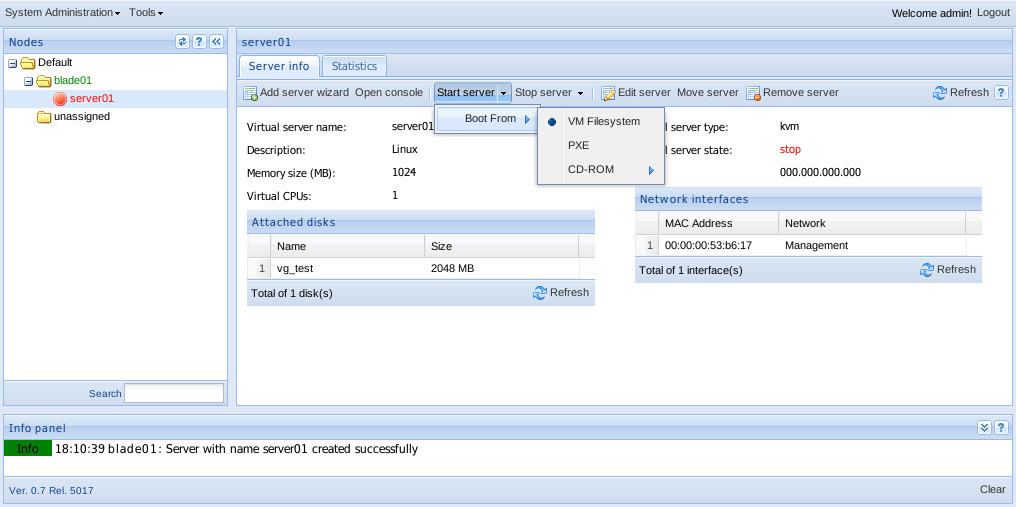
\includegraphics[scale=0.5]{screenshots/server_start.png}
	\caption{Migração de uma máquina virtual}
	\label{fig:server_migrate}
	\end{center}
\end{figure}


\subsection{Storage}
\label{sec:storage}

Em \emph{Storage} encontra-se a informação relativa aos volumes existentes no \emph{node}.
Este painel encontra-se divido em três secções:

\begin{description}
	\item[Devices -] Informação relativa aos \emph{physical volumes}\footnote{Um \emph{physical volume} é um dispositivo fisico, como por exemplo um disco} e seu estado. Permite fazer a administração de \emph{physical volumes} do \emph{node}.
	\item[Volume Groups -] Lista os \emph{volumes groups}\footnote{Um \emph{volume group} consiste na agregação de diversos \emph{physical volumes} num único volume virtual} existentes no node e seus \emph{physical volumes} associados. Permite fazer operações de administração de \emph{volume groups}.
	\item[Logical Volumes -] Apresenta a informação dos \emph{logical volumes}\footnote{Um \emph{logical volume} é uma "fatia" de um \emph{volume group}. É usado como sendo uma partição do sistema} do \emph{node}. Área de administração dos \emph{logical volumes}.
\end{description}


\begin{quote}
	{\large \bf Nota} \\*[-.8pc]
	\underline{\hspace{6in}} \\
	Existe um \emph{volume group} especial, \_\_DISK\_\_, utilizado no manuseamento de ficheiros. Esta etiqueta serve para, aquando da criação de um \emph{logical volume}, indicar que o disco a ser usado não é de facto um \emph{logical volume} mas sim um ficheiro.
\end{quote}


\begin{figure}[H]
	\begin{center}
	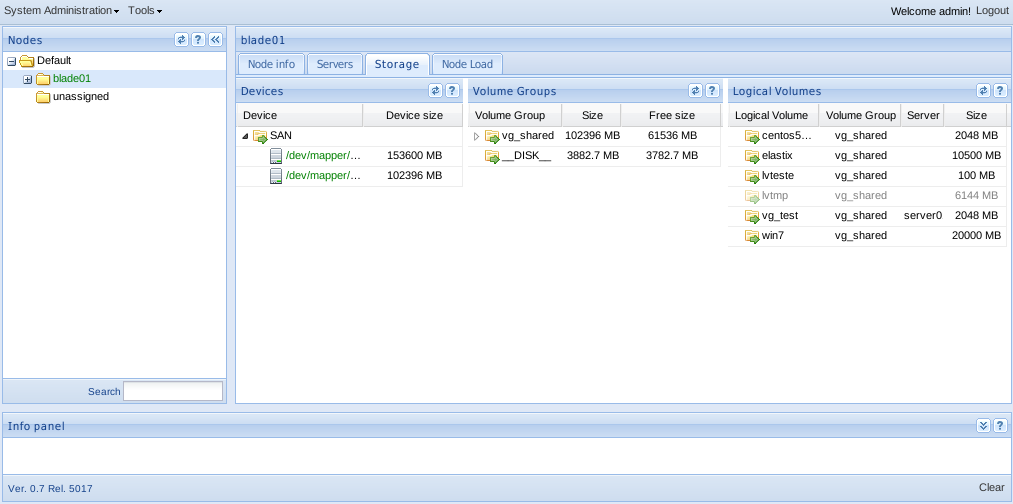
\includegraphics[scale=0.5]{screenshots/node_storage.png}
	\caption{Informação da Storage de um \emph{node}}
	\label{fig:inicial}
	\end{center}
\end{figure}

% ADMINISTRAÇÃO PHYSICAL VOLUMES

\subsubsection{Administração de Physical Volumes}
A administração de \emph{physical volumes} consiste nas seguntes operações:
\begin{itemize}
	\item Inicialização de um \emph{physical volume}
        \item Remoção de um \emph{physical volume}
\end{itemize}

\begin{figure}[H]
        \begin{center}
        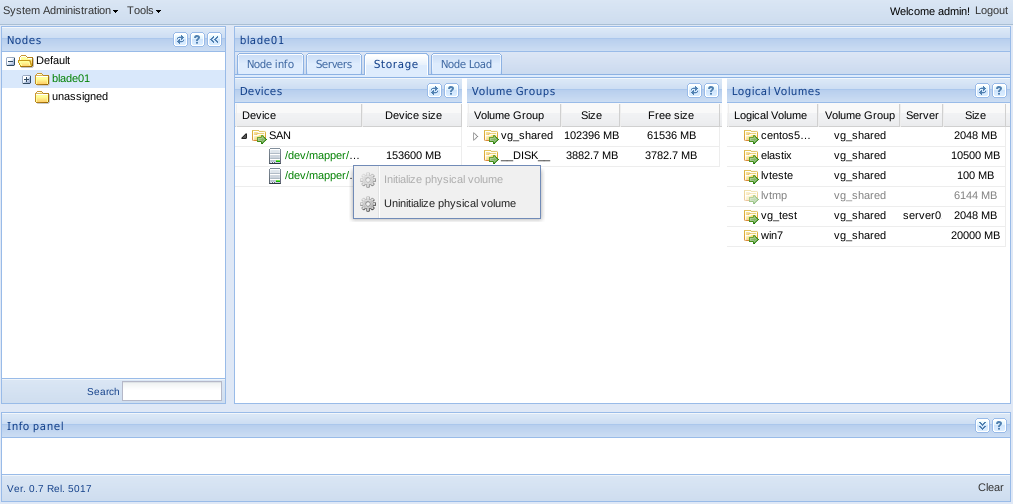
\includegraphics[scale=0.5]{screenshots/node_storage_device_ctx.png}
        \caption{Sub-menu de contexto de um physical volume}
        \label{fig:storage_device_ctx}
        \end{center}
\end{figure}


Para inicializar um \emph{physical volume} basta abrir o sub-menu de contexto do \emph{device} (clicar com o botão direito sobre o item) pretendido e seleccionar \emph{Initialize volume}. Para remover um \emph{physical volume} a operação é análoga bastando seleccionar a opção \emph{Uninitialize volume} no menu de contexto do \emph{physical volume}.

\begin{quote}
	{\large \bf Nota} \\*[-.8pc]
	\underline{\hspace{6in}} \\
	Só é permitido remover um \emph{physical volume} se este não pertencer a nenhum \emph{volume group}.
\end{quote}

% ADMINISTRAÇÃO VOLUME GROUPS

\subsubsection{Administração de Volume Groups}
Na administração de \emph{volumes groups} é permitido:
\begin{itemize}
	\item Criar um \emph{volume group}
	\item Extender um \emph{volume group}
	\item Reduzir um \emph{volume group}
	\item Remover um \emph{volume group}
\end{itemize}

\begin{figure}[H]
        \begin{center}
        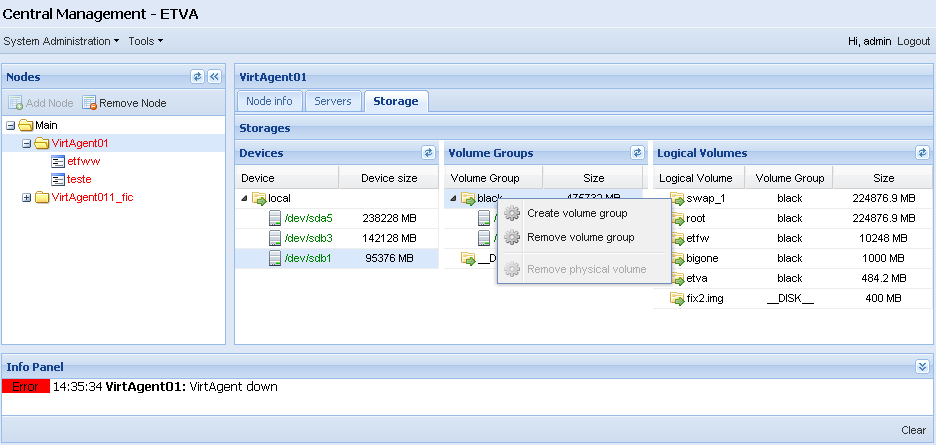
\includegraphics[scale=0.5]{screenshots/node_storage_vg_ctx.png}
        \caption{Sub-menu de contexto de um volume group}
        \label{fig:storage_vg_ctx}
        \end{center}
\end{figure}

Para criar um \emph{volume group} basta abrir o sub-menu de contexto sobre um qualquer \emph{volume group} e seleccionar \emph{Create volume group}.
Na janela de criação deverá ser introduzido o nome pretendido e seleccionar um ou mais \emph{physical voumes} disponiveis.

Um \emph{physical volume} está disponível quando não está alocado a um \emph{volume group} e encontra-se inicializado.

\begin{figure}[H]
        \begin{center}
        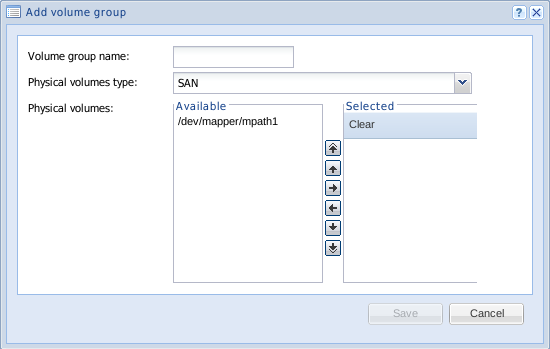
\includegraphics[scale=0.5]{screenshots/storage_vg_create.png}
        \caption{Janela de criação de um volume group}
        \label{fig:storage_vg_create}
        \end{center}
\end{figure}

Para extender um \emph{volume group} usa-se o \emph{drag-n-drop}, ou seja, arrasta-se o \emph{physical volume}, que se pretende adicionar, para cima do \emph{volume group} pretendido.

Na remoção/redução de um \emph{volume group} basta selecccionar o \emph{volume group}/\emph{physical volume} a remover e seleccionar a opção correspondente do sub-menu de contexto.
\begin{quote}
	{\large \bf Nota} \\*[-.8pc]
	\underline{\hspace{6in}} \\
	Só é permitido remover um \emph{volume group} se não houver nenhum \emph{logical volume} associado ao \emph{volume group}.
\end{quote}
 
\begin{figure}[H]
        \begin{center}
        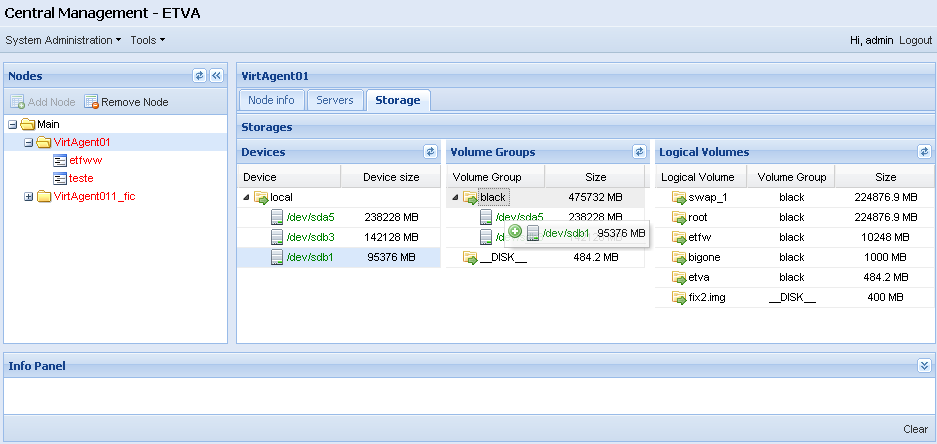
\includegraphics[scale=0.5]{screenshots/storage_vg_extend.png}
        \caption{Extensão de um volume group}
        \label{fig:storage_vg_extend}
        \end{center}
\end{figure}

Na figura \ref{fig:storage_vg_extend} extende-se o \emph{volume group} {\bf black} com o \emph{physival volume} {\bf sdb1}.

% ADMINISTRAÇÃO LOGICAL VOLUMES

\subsubsection{Administração de Logical Volumes}

As operações disponiveis sobre os \emph{logical volumes} são as seguintes:
\begin{itemize}
	\item Criar um \emph{logical volume}
	\item Redimensionar um \emph{logical volume}
	\item Remover um \emph{logical volume}
\end{itemize}

\begin{figure}[H]
        \begin{center}
        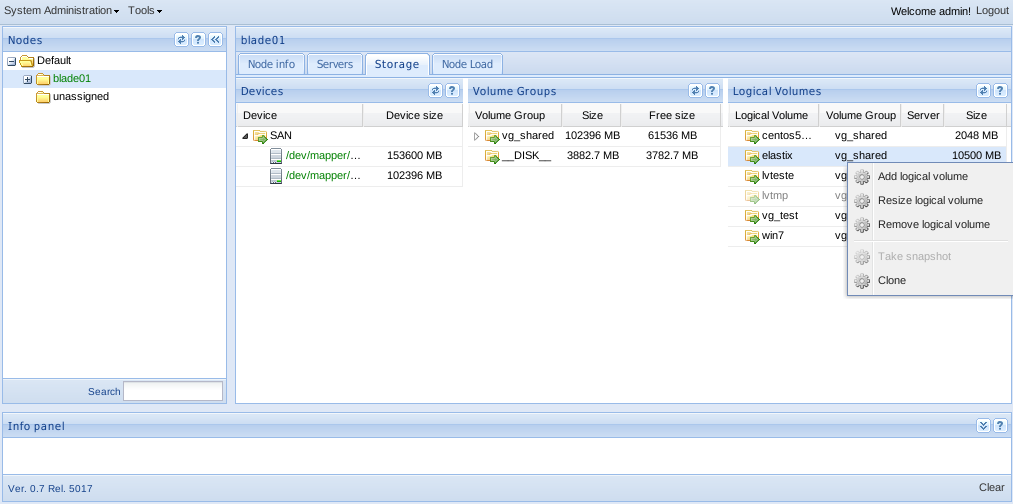
\includegraphics[scale=0.5]{screenshots/node_storage_lv_ctx.png}
        \caption{Sub-menu de contexto de um logical volume}
        \label{fig:storage_lv_ctx}
        \end{center}
\end{figure}

Para criar um \emph{logical volume} acede-se ao sub-menu de contexto sobre um qualquer \emph{logical volume} e selecciona-se \emph{Create logical volume}.
Na janela de criação deverá ser introduzido o nome pretendido, o \emph{volume group} a partir do qual se criará e o tamanho que não deverá exceder o tamanho disponível no \emph{volume group}.

\begin{figure}[H]
        \begin{center}
        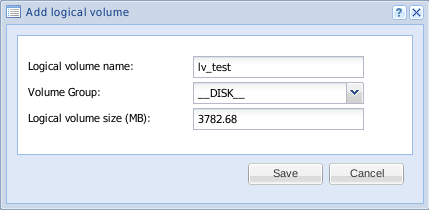
\includegraphics[scale=0.5]{screenshots/storage_lv_create.png}
        \caption{Janela de criação de um logical volume}
        \label{fig:storage_lv_create}
        \end{center}
\end{figure}

No redimensionamento selecciona-se o \emph{logical volume} que se pretende redimensionar e acede-se ao sub-menu de contexto. Aí existe a opção \emph{Resize logical volume} que permite aumentar/reduzir o tamanho do \emph{logical volume}.


\begin{quote}
	{\large \bf Nota} \\*[-.8pc]
	\underline{\hspace{6in}} \\
	Ao reduzir o tamanho do \emph{logical volume} poderá tornar os dados existentes inutilizados. É da responsabilidade do utilizador verificar se é comportável/seguro o redimensionamento do \emph{logical volume} sem afectar os dados nele contidos.
\end{quote}


\begin{figure}[H]
        \begin{center}
        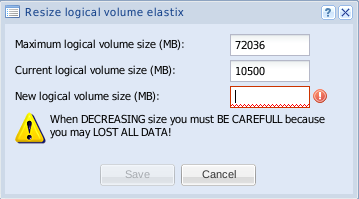
\includegraphics[scale=0.5]{screenshots/storage_lv_resize.png}
        \caption{Redimensionamento de um logical volume}
        \label{fig:storage_lv_resize}
        \end{center}
\end{figure}

Na remoção de um \emph{logical volume}, no sub-menu de contexto existe a opção \emph{Remove logical volume}. O \emph{logical volume} só será removido se não tiver associado a nenhuma máquina virtual. Para verificar se está em uso basta passar o rato por cima do \emph{logical volume} e observar a informação contida no \emph{tooltip} que aparece.

\pagebreak

\section{Máquinal virtual}
\label{sec:server}

No painel \emph{Nodes} é possível seleccionar a máquina virtual sobre o qual pretendemos efectuar operações como:

\begin{itemize}
        \item Gestão da máquina virtual
        \item Visualizar estatísticas
        \item Gestão das interfaces de rede da máquina virtual
        \item Gestão dos serviços do \emph{Management Agent}
\end{itemize}

\subsection{Server info}
Em \emph{Server Info} é disponibilizada a informação acerca do \emph{server}. Podemos ver o estado da máquina virtual e, entre outras informações, o estado do \emph{Management Agent}.
Para além de visualizar informação, este painel permite efectuar as seguintes operações:
\begin{itemize}
	\item Adicionar máquina virtual (ver secção \ref{sec:add_server})
	\item Remover máquina virtual (ver secção \ref{sec:remove_server})
	\item Abrir máquina virtual numa consola VNC (ver secção \ref{sec:open_vnc})
	\item Iniciar/parar máquina virtual (ver secção \ref{sec:start_server})
    \item Migrar máquina virtual (ver secção \ref{sec:start_server})
\end{itemize}

\begin{figure}[H]
	\begin{center}
	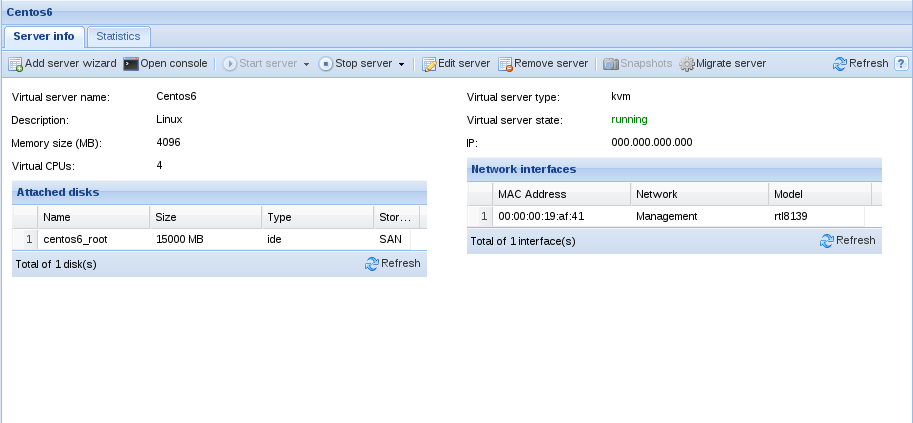
\includegraphics[scale=0.5]{screenshots/server_info.png}
	\caption{Informação da máquina virtual \emph{etfww}}
	\label{fig:server_info}
	\end{center}
\end{figure}

\subsection{Statistics}
Em \emph{Statistics} é possível visualizar gráficamente informação de:
\begin{itemize}
	\item Cpu Usage
	\item Networks
	\item Memory Usage
	\item Disk
	\item Node Load
\end{itemize}


\begin{figure}[H]
	\begin{center}
	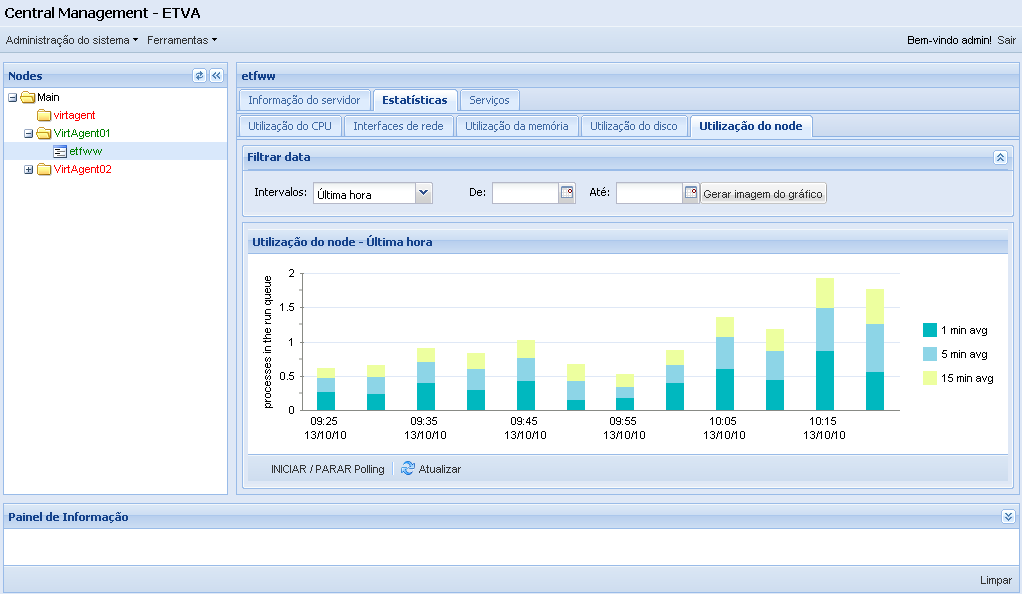
\includegraphics[scale=0.5]{screenshots/server_stats_nodeLoad.png}
	\caption{Estatisticas de uma máquina virtual}
	\label{fig:server_stats_nodeLoad}
	\end{center}
\end{figure}

Em cada um destes paineis é possível visualizar os dados pelos \emph{presets} existentes:
\begin{itemize}
	\item Last day
	\item Last Hour
	\item Last 2 hour
	\item Last week
\end{itemize}

Na figura \ref{fig:server_stats_nodeLoad}, visualiza-se a informação de carga do node a que pertence o server \emph{etfww} para no preset - \emph{Last day}

Para visualizar outros intervalos de tempo(Date Range) usa-se \emph{Generate graph image}.
\begin{figure}[H]
	\begin{center}
	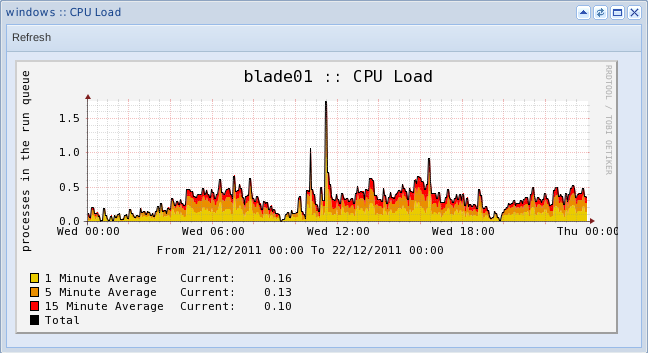
\includegraphics[scale=0.5]{screenshots/server_stats_nodeLoadRange.png}
	\caption{Estatisticas de \emph{Node Load} pdo node \emph{VirtAgent01} - Date Range}
	\label{fig:server_stats_nodeLoadRange}
	\end{center}
\end{figure}

\subsection{Networks}

Em \emph{Networks} é possível gerir as interfaces de rede associadas ao server.
Permite remover uma NIC - \emph{Remove NIC}, ou alterar as NIC's existentes - \emph{Add NIC}

\begin{figure}[H]
	\begin{center}
	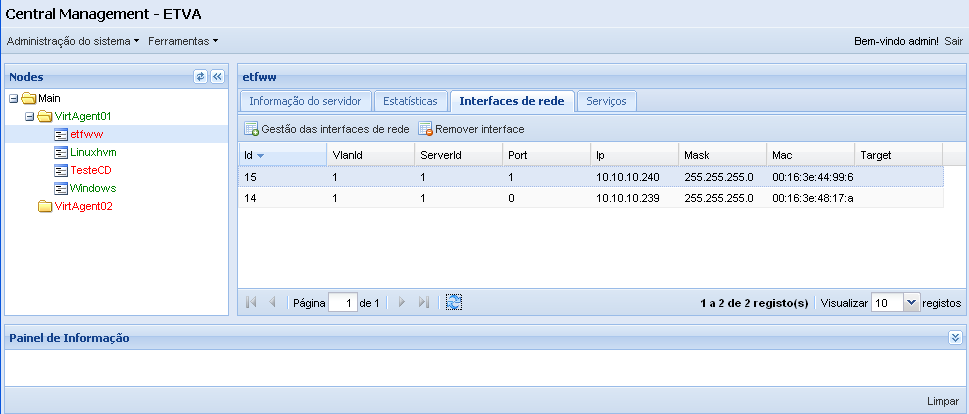
\includegraphics[scale=0.5]{screenshots/server_networks.png}
	\caption{Lista das interfaces de um server}
	\label{fig:server_networks}
	\end{center}
\end{figure}



\subsection{Services}
Em \emph{Services}, e caso esteja configurado um MA (\emph{Management Agent}) no \emph{server}, é disponibilizada a respectiva configuração dos serviços controlados por esse MA.
